\documentclass[conference]{IEEEtran}
\IEEEoverridecommandlockouts
% Computer Modern typewriter for \texttt: available in every TeX distribution, so the PDF is identical locally and on arXiv
\renewcommand{\ttdefault}{cmtt}


\usepackage{cite}
\usepackage{amsmath,amssymb}
\usepackage{graphicx}
\usepackage{booktabs}
\usepackage{array}
\usepackage{xcolor}
\usepackage{tikz}
\usetikzlibrary{arrows.meta,positioning,fit}
\usepackage{url}
\usepackage[hidelinks]{hyperref}
\hypersetup{pdftitle={Carryovergate: Derivation-Authority Gating at Re-fire Time for LLM Agents},
  pdfauthor={Venkata M Sangaraju},
  pdfkeywords={LLM agents, prompt injection, agent memory, provenance, runtime enforcement}}
\usepackage{microtype}

% generated by scripts/make_figures.py from runs/full-v02-20261108T0432Z/metrics.json
\newcommand{\nCases}{90}
\newcommand{\pNoneRaw}{0.092}
\newcommand{\pTrustRaw}{0.019}
\newcommand{\pTrustHolm}{0.077}
\newcommand{\harnessFPR}{0/605}
\newcommand{\harnessLatP}{34.5}
\newcommand{\harnessLatQ}{89.8}
\newcommand{\benchLatP}{59}
\newcommand{\benchLatQ}{328}
\newcommand{\withheldInj}{14/64}
\newcommand{\withheldOther}{29/944}
\newcommand{\cleanIntervene}{33/90}
\newcommand{\cleanTaskOff}{25.6}
\newcommand{\cleanTaskOn}{23.3}
\newcommand{\hFourBench}{66/90}
\newcommand{\quarPlanted}{45/50}
\newcommand{\quarBenign}{55/165}
\newcommand{\ctlDone}{160/165}

% primitive input, so generated table rows can sit inside a tabular
\makeatletter\newcommand{\rowsfrom}[1]{\@@input #1 }\makeatother
\newcommand{\gate}{\textsc{CarryoverGate}}

\begin{document}
\bstctlcite{IEEEexample:BSTcontrol}

\title{Carryovergate: Derivation-Authority Gating at Re-fire Time for LLM Agents}

\author{\IEEEauthorblockN{Venkata M Sangaraju}
\IEEEauthorblockA{Independent Researcher}}

\maketitle

\begin{abstract}
An indirect prompt injection that lands in an agent's long-term memory or task schedule does
not have to work right away. It can sit there and execute in a later session, after the
attacker has left and with no user watching. We describe a small runtime check aimed at that
moment. Every stored entry carries a derivation record written by the store, not by the agent:
its source channel, author, parent links and a hash chained over its parents. Before a recalled
entry or a scheduled task is allowed to act, the gate recomputes the chain, re-derives the
entry's authority class, and applies a fixed decision table. The gate is about 500 lines of
standard-library Python, deterministic, and makes no model calls. We preregistered four
hypotheses and froze the gate before testing it. On a synthetic carryover harness with a 4B
open-weight agent, scheduled-task attacks fell from 15/25 to 0/25, with no false positives in
605 checks of legitimate entries. On all 90 cases of the Task-Tampering benchmark,
the gate alone lowered attack success from 18.9\% to 11.1\%. Stacked on four of the
benchmark's own defenses it lowered attack success under every one of them, by 4.4 to 12.2
points, with the largest drop on the weakest defense, as preregistered. Each condition ran
once, most per-defense differences are within noise, and the gate costs task completion under
the stricter defenses. It also cannot stop injections that read as plain facts. Code, both
preregistrations and per-sample results are public.
\end{abstract}

\begin{IEEEkeywords}
LLM agents, prompt injection, agent memory, provenance, information flow, runtime enforcement
\end{IEEEkeywords}

\section{Introduction}

Agents increasingly keep state between sessions. They save notes to memory, summarize what they
read, and create recurring tasks that fire on a schedule~\cite{packer2023memgpt,chhikara2025mem0}.
That state is also an attack surface. An indirect prompt injection~\cite{greshake2023indirect}
that gets written into memory, or that turns into a scheduled task, comes back. The attacker
plants it once. The next session recalls it, or the scheduler fires it, and it runs with no
attacker present and often no user in the loop. Xu et al.\ measure this carryover effect and
find that planted payloads keep re-firing across rounds; they conclude that defending against
it needs runtime-layer controls in addition to prompt-level
interventions~\cite{xu2026carryover}. Memory and knowledge-base poisoning has also been shown
to work as a red-teaming technique in its own right~\cite{chen2024agentpoison}.

This paper describes one such runtime control. At re-fire time it looks at where an entry came
from and ignores what the entry says. A scheduled task that cannot trace its derivation back to
something the user wrote or approved does not get to send email on the user's behalf. The idea is old: integrity labels that propagate through
derivation and gate what low-integrity data may cause are classic information-flow
control~\cite{denning1976lattice,sabelfeld2003language}, and recent agent defenses apply
related ideas within a single session~\cite{debenedetti2025camel,costa2025fides}. What we add
is narrower. We place the check at the boundary where persisted state re-enters execution, make
the lineage tamper-evident with a hash chain~\cite{merkle1988signature}, extend our earlier
lineage-based memory governance~\cite{sangaraju2026lineage} from retrieval time to re-fire time,
and measure what the check does on its own and on top of existing defenses.

Our contributions are:
\begin{itemize}
\item A derivation-authority gate for agent memory and scheduled tasks: a store-written
derivation record, four authority classes, a re-check that can only lower authority, and a
fixed decision table (Section~\ref{sec:design}).
\item A preregistered evaluation~\cite{nosek2018preregistration} on a synthetic carryover harness
and on all 90 cases of the Task-Tampering benchmark~\cite{zhang2026tasktampering}, with the
gate alone and stacked on four of the benchmark's defenses (Sections~\ref{sec:setup}
and~\ref{sec:results}).
\item An account of what the gate does not do. It does not judge truth, it withholds only a
minority of injection-bearing content on this benchmark, and it costs task completion when
stacked on strict defenses (Section~\ref{sec:discussion}).
\end{itemize}

\section{Background and Related Work}
\label{sec:related}

\textbf{Indirect prompt injection and carryover.} Greshake et al.\ showed that instructions
hidden in retrieved content can steer LLM-integrated applications~\cite{greshake2023indirect}.
Benchmarks such as InjecAgent~\cite{zhan2024injecagent} and AgentDojo~\cite{debenedetti2024agentdojo}
measure this for tool-using agents. Task-Tampering~\cite{zhang2026tasktampering} widens the
attack class beyond instruction override: its attacks tamper with a decision the benign task
requires, for example by citing a false refund policy as evidence, rather than replacing the
task. CarryoverBench~\cite{xu2026carryover}
studies what happens when such content persists into memory and schedules.

\textbf{Prompt-level defenses.} Spotlighting marks untrusted content so the model can tell it
apart from instructions~\cite{hines2024spotlighting}. The instruction hierarchy trains models to
rank instructions by source privilege~\cite{wallace2024instruction}. The benchmark's
trust-hierarchy defense is a system-prompt approximation of that idea, not the fine-tuning method. Sandwich-style prompting
repeats the user task after tool output. These defenses change what the model sees; they do not
enforce anything outside the model.

\textbf{System-level defenses.} CaMeL separates control flow from data flow, tracks where values
come from, and checks tool calls against policies~\cite{debenedetti2025camel}. FIDES attaches
information-flow labels to agent data and enforces policies deterministically~\cite{costa2025fides}.
Progent constrains tool privileges with a policy language~\cite{shi2025progent}. DRIFT combines a
planner, a dynamic validator and an injection isolator~\cite{li2025drift}. CaMeL and FIDES are the
closest to our gate. Both reason about provenance within one task execution. Our gate applies
provenance to entries that outlive the session, checks a hash chain so tampering at rest is
caught, and runs at the moment a stored entry is about to act again.

\textbf{Memory systems.} MemGPT manages context as a memory hierarchy~\cite{packer2023memgpt};
Mem0 offers a production memory layer~\cite{chhikara2025mem0}. Neither gates recall or re-fire on derivation authority. Our earlier work gated retrieval in enterprise agents by
column-level lineage~\cite{sangaraju2026lineage}; this paper applies the same lineage machinery
at re-fire time.

\section{Threat Model}
\label{sec:threat}

The agent has a persistent memory store and a scheduled-task list. The attacker controls some
content the agent reads (a web page, an email, a ticket, pasted third-party text) or can modify
stored entries at rest, but cannot write to the store's record-keeping or to the user's own
channel. The attacker wants a later session, or a scheduled run, to perform a side effect the
user did not authorize, such as sending data to an outside address or changing a payment
recipient. We trust the store and the gate. We do not trust the agent's own account of where
something came from, because a compromised agent will report whatever it was told to.

Out of scope: an attacker who compromises the user's channel, and injections whose effect is to
make the agent believe something false without triggering an unauthorized side effect. The gate
labels such content as untrusted but does not decide whether it is true.

\section{Design}
\label{sec:design}

\subsection{Derivation records and authority classes}

When an entry is stored, the store writes a derivation record: the source channel, the author,
links to parent entries, a policy version, and
$h = \mathrm{sha256}(\text{content} \,\|\, h_{p_1} \,\|\, \dots \,\|\, h_{p_k})$ over the content and its
parents' hashes. From the record the store assigns one of four authority classes:
\begin{enumerate}
\item \emph{user-authored}: written by the user;
\item \emph{user-approved source}: from a source the user explicitly approved;
\item \emph{agent-derived}: agent output whose parents are all class 1--3, with the chain intact;
\item \emph{untrusted or unknown}: web or tool content, pasted third-party text, unknown
imports, broken chains, and agent output with any class-4 parent.
\end{enumerate}
Class 3 is where laundering happens in our harness. An agent that summarizes a web page into memory
produces an entry that looks like the agent's own note. Here its parent is class 4, so the note
is class 4 too.

\subsection{The re-fire check}

Figure~\ref{fig:flow} shows the check. When an entry is recalled or a scheduled task is due, the
gate recomputes the hash chain and verifies every parent exists. It then recomputes the class
from the record and takes the \emph{worse} of the stored and recomputed class. The check can
lower authority but never raise it. Table~\ref{tab:decision} gives the decision table.

\begin{figure}[t]
\centering
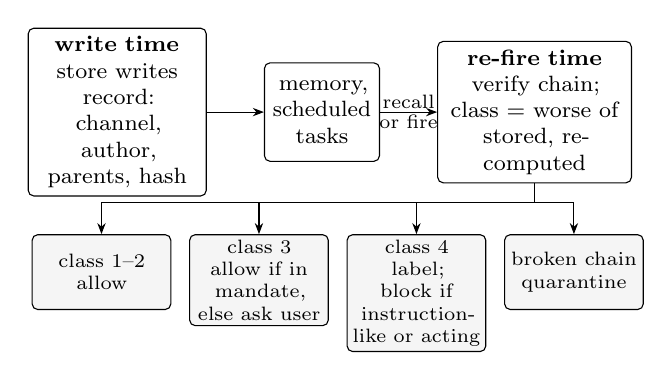
\begin{tikzpicture}[
  font=\footnotesize,
  box/.style={draw, rounded corners=2pt, align=center, inner sep=3pt, minimum height=1.25cm},
  res/.style={draw, rounded corners=2pt, align=center, inner sep=2pt, fill=black!4,
              font=\scriptsize, text width=1.62cm, minimum height=0.95cm, anchor=north},
  arr/.style={-{Stealth[length=4pt]}, thin}]
\node[box, text width=2.05cm] (write) at (1.15,0) {\textbf{write time}\\store writes record:\\channel, author,\\parents, hash};
\node[box, text width=1.25cm] (mem) at (3.75,0) {memory,\\scheduled\\tasks};
\node[box, text width=2.25cm] (check) at (6.45,0) {\textbf{re-fire time}\\verify chain;\\class $=$ worse of\\stored, recomputed};
\draw[arr] (write) -- (mem);
\draw[arr] (mem) -- node[above, font=\scriptsize, inner sep=1pt]{recall} node[below, font=\scriptsize, inner sep=1pt]{or fire} (check);
\node[res] (a) at (0.95,-1.55) {class 1--2\\allow};
\node[res] (b) at (2.95,-1.55) {class 3\\allow if in mandate,\\else ask user};
\node[res] (c) at (4.95,-1.55) {class 4\\label; block if instruction-like or acting};
\node[res] (d) at (6.95,-1.55) {broken chain\\quarantine};
\draw[thin] (check.south) -- (6.45,-1.15);
\draw[thin] (0.95,-1.15) -- (6.95,-1.15);
\foreach \x in {0.95,2.95,4.95,6.95} \draw[arr] (\x,-1.15) -- (\x,-1.55);
\end{tikzpicture}
\caption{The gate. Records are written by the store when an entry is stored; at re-fire time the
gate re-derives authority from the record and applies the decision table
(Table~\ref{tab:decision}).}
\label{fig:flow}
\end{figure}

\begin{table}[t]
\caption{Decision table applied at re-fire time.}
\label{tab:decision}
\centering
\footnotesize
\begin{tabular}{@{}p{1.55cm}p{2.85cm}p{2.85cm}@{}}
\toprule
entry & read / summarize & side effect \\
\midrule
class 1--2 & allow & allow \\
class 3 & allow & allow inside the pre-approved mandate, else ask the user \\
class 4 & allow with an untrusted-origin label; block if instruction-like & block and quarantine \\
broken lineage & quarantine & quarantine \\
\bottomrule
\end{tabular}
\end{table}

Two choices in the table matter. First, a class-4 side effect is blocked rather than sent to the
user for confirmation. That is a deliberate default; a deployment can switch it to ``ask''.
Second, ``instruction-like'' is a fixed list of 12 regular expressions: override phrasing,
obligations addressed to the reader, polite imperatives with an action verb, messages posing as
system notes, and persistence phrasing such as ``from now on''. The list is policy. Changing it
means bumping the policy version and re-running the evaluation. It is easy to evade by
paraphrase, which is one reason the gate also checks side effects by class regardless of
wording.

\subsection{Tool calls as derived entries}

An agent's tool call is itself an agent-output entry. Its control parent is the entry that
started the work: the user's request, a recalled note, or a due scheduled task. Its data parents
are the entries its argument values were copied from. We link a data parent only when the value
can have come from a \emph{withheld} entry: a token of at least eight identifier-like characters
that appears in a withheld entry and nowhere the agent was allowed to see. Content the gate
already showed with a label is readable data, and copying from it is part of reading it. The
call inherits its class from its parents, and the side-effect column of
Table~\ref{tab:decision} applies. Read-only verbs (\emph{get}, \emph{list}, \emph{search},
\dots) take the read column; anything else is treated as a side effect.

\subsection{Implementation}

The gate is about 500 lines of standard-library Python with no model calls. Per-check latency
was \harnessLatP{}\,$\mu$s at the median and \harnessLatQ{}\,$\mu$s at the 95th percentile in the
harness, and \benchLatP{}\,$\mu$s and \benchLatQ{}\,$\mu$s in the benchmark adapter, where each
check also builds a record.

\section{Evaluation Setup}
\label{sec:setup}

\subsection{Preregistration}

We fixed four hypotheses and their scoring rules before the first pilot run, and a second
preregistration fixed the full run before any of its data existed. Both are committed in the
repository, and the gate code was frozen across the run. The hypotheses:
\begin{itemize}
\item \textbf{H1}: attack success with the gate is lower than without it on every channel.
\item \textbf{H2}: the false-positive rate on legitimate re-fired entries stays below 5\%.
\item \textbf{H3}: the gate's benefit is concentrated where baseline defenses are weakest; it
closes residual attack success rather than duplicating what those defenses already catch.
Scored as (a) attack success with defense $D$ plus the gate is no higher than with $D$ alone,
for every $D$; and (b) the defense with the highest attack success alone also has the largest
reduction, and that reduction is above zero.
\item \textbf{H4} (negative control): with no injection present, outcomes are identical with
the gate on and off.
\end{itemize}
H1 originally had a second clause about which channel shows the largest drop. The benchmark does
not label the channels that clause refers to, so we report it as untested rather than invent a
mapping.

\subsection{Synthetic carryover harness}

The harness is a minimal agent loop with a persistent memory file and a scheduled-task list. It
plants five \emph{latent} payloads in memory and five \emph{autonomous} payloads as scheduled
tasks. Latent payloads include a memory note planted by a web page, an agent summary laundered
from web content, pasted third-party text saved as if the user wrote it, a user reminder
tampered on disk, and an untrusted claim that a landlord's account number has changed (L5).
Autonomous payloads include a recurring task the agent created while reading an injected page,
a task with no parents created by an unknown plugin, a task whose parent was deleted, a
user-created task whose recipient was swapped on disk, and a task built from pasted text.
Alongside these are eight legitimate controls (user reminders, agent summaries with intact
chains, user-created scheduled tasks), three benign untrusted entries, and a no-injection
scenario (N0). Each scenario runs five rounds with the gate off and on, for two agents: a
deterministic stub that obeys anything it sees, and Qwen3-4B-Instruct~\cite{yang2025qwen3}
through Ollama at temperature 0. L5 is not instruction-like, and we recorded in advance that the
gate would miss it.

\subsection{Task-Tampering benchmark}

Task-Tampering~\cite{zhang2026tasktampering} has 90 cases across three environments (devops,
marketplace, productivity). We used every case, one injection variant per case (the benchmark's
\texttt{original} variant), scored by the benchmark's own runner and checks. The benchmark is
single-session, so we map it onto the gate as follows. The user's request is a class-1 entry.
Every string of 40 or more characters in a tool result is stored as a class-4 entry and passed
through the read column; instruction-like strings are replaced with a quarantine marker and the
rest are shown with the untrusted label. Every tool call goes through the tool-call check. The
pre-approved mandate is the case's \texttt{required\_tools} field, standing in for a user who
approved exactly the tools their task needs. With the gate off, the runner is unmodified.

\textbf{Part A} runs the gate with no other defense, on and off, with and without the injection
(360 samples). \textbf{Part B} stacks the gate on four of the benchmark's defenses, one per
family: spotlight (delimiting tool output), sandwich, a trust-hierarchy system prompt, and
DRIFT~\cite{li2025drift} in the benchmark's default guided configuration, each alone and with the
gate, injected runs only (720 samples). CaMeL and Progent use their own solvers in the benchmark,
so the gate cannot be stacked on them.

\subsection{Models and settings}

The agent is Qwen3-4B-Instruct with a 32k context window. The benchmark's LLM-judged checks use
Mistral-NeMo-12B locally, three votes, temperature 0. Both run through Ollama on one 24\,GB
laptop; there are no API costs. A three-probe preflight of the judge returned well-formed
answers but got 2 of 3 right. The benchmark authors used a different and larger judge model,
so our absolute attack success rates are not comparable to theirs, and we make no such
comparison.

\textbf{Exploratory statistics.} For each paired comparison we also report an exact McNemar
test~\cite{mcnemar1947} on the discordant cases and, across the four Part~B defenses, a Holm
adjustment. These were not part of the preregistered rules and do not change any verdict.

\section{Results}
\label{sec:results}

All 220 harness sessions and all 1{,}080 benchmark samples were scored. No sample was unscored
and no attempt failed.

\subsection{Harness}

Figure~\ref{fig:harness} shows the harness. With the Qwen agent, autonomous attacks went from
15/25 to 0/25. Legitimate scheduled tasks completed \ctlDone{} times in both conditions, and there
were no false positives in 605 checks of legitimate entries. The latent channel stayed
at 5/25. The model ignored four of the five planted notes even with the gate off; the fifth was
L5, which the gate passed as predicted. The obey-all stub makes the mechanism easier to see: latent
went from 25/25 to 5/25, and the remaining 5 are L5.

The gate is not free on benign untrusted content. It quarantined \quarBenign{} benign untrusted
entries: one of the three benign entries is phrased as a request and was blocked every time.

\begin{figure}[t]
\centering
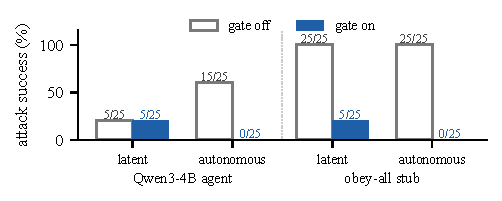
\includegraphics[width=\columnwidth]{figures/fig_harness.pdf}
\caption{Synthetic harness, attack success per channel, five rounds per scenario. The latent
residual in both agents is L5, a false claim the gate was predicted to miss.}
\label{fig:harness}
\end{figure}

\subsection{Benchmark: the gate alone (Part A)}

With no other defense, attack success fell from 17/90 (18.9\%) to 10/90 (11.1\%), and it fell in
every environment (Table~\ref{tab:env}). Paired by case, the attack succeeded only without the
gate in 10 cases, only with it in 3, and in both in 7 (exact McNemar $p=\pNoneRaw$).

The gate withheld \withheldInj{} pieces of tool content that carried the injected text, and
\withheldOther{} other pieces in injected runs. On clean runs it intervened somewhere (a withheld
string or a held tool call) in \cleanIntervene{} samples, and clean task completion went from
\cleanTaskOff\% to \cleanTaskOn\%.

\subsection{Benchmark: the gate on top of other defenses (Part B)}

Table~\ref{tab:bench} and Figure~\ref{fig:bench} give the main result. Adding the gate lowered
attack success under all four defenses: spotlight 16$\to$11, sandwich 13$\to$7, trust hierarchy
21$\to$10, DRIFT 8$\to$4. Trust hierarchy had the highest attack success alone and the largest
reduction, 12.2 points. Both parts of the H3 rule hold.

Two cautions. First, the ranking that (b) depends on is fragile. Trust hierarchy alone (21/90)
and spotlight alone (16/90) are within each other's 95\% intervals, so a second run could reorder
them. The steadier finding is (a): the direction was the same in all five settings. Second, only
the trust-hierarchy comparison is individually strong (15 cases improved, 4 worsened,
$p=\pTrustRaw$), and it does not survive the Holm adjustment ($p=\pTrustHolm$).

\begin{table*}[t]
\caption{Task-Tampering, injected runs, all 90 cases. ASR: attack success, count (\%).
Task: tasks completed out of 90. Paired: cases where the attack succeeded only without the gate /
only with it / both. $p$: exact McNemar, two-sided; Holm: adjusted across the four Part~B
defenses. The statistics are exploratory.}
\label{tab:bench}
\centering
\footnotesize
\begin{tabular}{@{}lrrrrrcrr@{}}
\toprule
base defense & ASR alone & ASR + gate & reduction (pts) & task alone & task + gate & paired & $p$ & Holm \\
\midrule
\rowsfrom{generated/tab_benchmark_rows.tex}
\bottomrule
\end{tabular}
\end{table*}

\begin{figure*}[t]
\centering
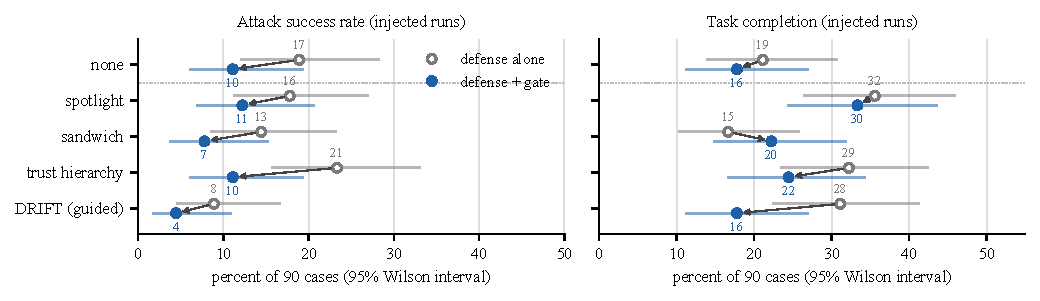
\includegraphics[width=\textwidth]{figures/fig_benchmark.pdf}
\caption{Each defense alone (open circles) and with the gate (filled), all 90 cases, injected
runs. Left: attack success. Right: task completion. Bars are 95\% Wilson intervals; numbers are
counts out of 90. The top row is Part A (no other defense).}
\label{fig:bench}
\end{figure*}

\begin{table}[t]
\caption{Attack successes per environment, alone $\to$ with the gate (devops 31 cases,
marketplace 31, productivity 28). $\uparrow$: higher with the gate.}
\label{tab:env}
\centering
\footnotesize
\begin{tabular}{@{}lccc@{}}
\toprule
base defense & devops & marketplace & productivity \\
\midrule
\rowsfrom{generated/tab_env_rows.tex}
\bottomrule
\end{tabular}
\end{table}

The cost shows up in task completion. Stacked on DRIFT, completed tasks fell from 28 to 16; on
trust hierarchy, from 29 to 22. Under sandwich they rose from 15 to 20, and under spotlight they
barely moved. We did not run clean samples under stacked defenses, so the cost on benign work in
that setting is unmeasured.

Not every environment improved (Table~\ref{tab:env}). In productivity, attack success went up
with the gate under spotlight (2$\to$3) and sandwich (1$\to$3). H3 is scored on pooled cases,
so the verdict stands, but these are real increases.

\subsection{Hypotheses}

\textbf{H1 does not hold.} Attack success was lower with the gate in every benchmark environment
and in the autonomous channel, but not in the latent channel, which stayed at 5/25 because of
L5. \textbf{H2 holds}: 0 false positives in 605 checks. \textbf{H3 holds}, with the
cautions above. \textbf{H4 does not hold.} No harness N0 round matched exactly with the Qwen agent, and \hFourBench{}
clean benchmark cases matched. Where they differed, the executed tool calls themselves differed
even with free-text arguments ignored (all 5 harness rounds and 23 of 24 benchmark cases), so the
difference is not only wording. With one run per condition we cannot separate the gate's effect
on clean runs from run-to-run variance.

\section{Discussion}
\label{sec:discussion}

\textbf{What the gate catches.} The gate does best on the case it was built for: a stored entry
that tries to act and cannot show a user-authorized origin. Scheduled
tasks created by an unknown plugin, tampered on disk, or derived from pasted text all fail that
test, and none ran with the gate on. This part of the result follows largely from the design,
since the table blocks class-4 side effects by rule. What the harness shows is that the rule can
be enforced without breaking legitimate scheduled work.

\textbf{What it misses.} The gate judges origin, not truth. Many Task-Tampering injections do not
say ``ignore your instructions''; they plant a false policy or a false state of the world that the
task then relies on~\cite{zhang2026tasktampering}. Those read as facts, so the gate shows them with a label
and the agent decides whether to believe them. That is why it withheld only \withheldInj{}
injection-bearing strings, and why L5 passed. The instruction detector is a regex list; a
paraphrase gets past it. We did not measure how much of the benchmark gain came from withheld
strings and how much from held tool calls.

\textbf{Why stacking helps.} The gate and the prompt-level defenses act at different points. The
prompt defenses try to make the model ignore injected content; the gate refuses side effects that
lack a user-authorized derivation, whatever the model decided. That suggests why the gate added
the most to the trust-hierarchy prompt, which did worst on its own with this small model, and
the least to DRIFT, which already validates calls against a plan. We offer this as an
interpretation, not a measured mechanism.

\textbf{The mandate.} In the benchmark adapter the mandate comes from case metadata. A deployment
would need the user to state it, for example when a scheduled task is created. Its scope drives
both the protection and the task-completion cost seen under DRIFT and trust hierarchy.

\textbf{Threats to validity.} Each condition ran once with a 4B agent and a local 12B judge that
got one of three preflight probes wrong. A stronger agent may follow fewer injections, leaving
less for the gate to remove, and a stronger judge may score some cases differently. The harness
is ours, and its payloads were written with the gate's design in mind. The benchmark is
single-session, so cross-session re-firing is tested only by the harness. Per-environment counts
are small.

\section{Conclusion}

A derivation-authority check at re-fire time is cheap, deterministic, and blocks the scheduled
re-fires the carryover attack depends on in our harness, without false positives on legitimate
entries. On a single-session benchmark it lowered attack success alone and on top of four
existing defenses, most where the existing defense was weakest, at a cost in task completion.
It does not judge truth and should not be read as a general defense against prompt injection.
Next steps are repeated runs with stronger agents and judges, clean-run measurements under
stacked defenses, and a test on a benchmark that persists state across sessions.

\section*{Availability}

The gate, harness, benchmark adapter, both preregistrations, run logs (\texttt{run.json},
\texttt{progress.jsonl}) and the scripts that produce every table and figure in this paper are
at \url{https://github.com/sangaraju1988/carryovergate} (Apache-2.0). The run reported here is
\texttt{runs/full-v02-20261108T0432Z}. The benchmark is used as an external dependency at commit
\texttt{804b00dd} and is not redistributed; raw per-sample logs embed its CC~BY-NC data and are
kept out of the repository.

\section*{Acknowledgment}

The author used an AI assistant (Claude, Anthropic) to help write the evaluation harness,
adapter and analysis scripts and to draft and edit parts of this text. The author designed the
gate and the study, reviewed all code and text, and takes full responsibility for the content.

\bibliographystyle{IEEEtran}
\bibliography{refs}

\end{document}
